\documentclass[11pt,a4paper]{article}
\usepackage[margin=0.85in]{geometry}
\usepackage{graphicx,booktabs,array,longtable,float,caption,xcolor,hyperref}
\usepackage[T1]{fontenc}
\usepackage{lmodern}
\hypersetup{colorlinks=true,linkcolor=blue,urlcolor=blue}
\setlength{\parskip}{5pt}
\setlength{\parindent}{0pt}
\renewcommand{\arraystretch}{1.18}
\title{Exploratory Data Analysis and Feature Engineering Report\\\large Phase 3 --- Household Electricity Bill Forecasting}
\author{}
\date{}
\begin{document}
\maketitle
\vspace{-1.2cm}
\section{Introduction and Dataset Overview}
\subsection{Introduction}
Predicting household electricity bills before the end of a billing cycle can help consumers anticipate costs and manage energy usage. Smart-meter data provides an opportunity to develop such predictions using historical consumption patterns.

This phase focuses on exploratory data analysis (EDA) and feature engineering to identify consumption trends, relationships, outliers, and relevant forecasting features. The analysis supports the project's research question:

\textbf{How accurately can a household's upcoming electricity bill be predicted using historical smart-meter consumption data?}
\subsection{Dataset Overview}
The study uses the Low Carbon London smart-meter dataset, previously processed into monthly household observations from half-hourly electricity readings. The processed data also includes tariff, household classification, and temperature information.
\begin{table}[H]\centering\caption{Dataset overview}\small
\begin{tabular}{@{}p{0.39\linewidth}p{0.54\linewidth}@{}}\toprule
Characteristic & Description\\\midrule
Data source & Low Carbon London Smart Meter Dataset\\
Study period & December 2011--January 2014\\
Observations & 106,225 household-month records\\
Unique households & 5,548\\
Original processed dataset & \texttt{monthly.parquet}\\
Previously encoded dataset & \texttt{monthly\_encoded.parquet} (15 columns)\\
Phase 3 engineered dataset & \texttt{monthly\_features.parquet} (23 columns)\\\bottomrule
\end{tabular}\end{table}
The principal variables include monthly electricity consumption (\texttt{kwh}), estimated electricity bills (\texttt{bill\_gbp}), tariff category, ACORN household classification, mean temperature, and calendar information. The prediction target is \texttt{bill\_gbp}.
\subsection{Scope}
This phase examines descriptive statistics, data distributions, seasonal patterns, correlations, and outliers. It also introduces historical consumption and calendar-based features while retaining categorical indicators encoded during Phase 2.

Current-month total consumption is excluded as an advance forecasting predictor to prevent target leakage. Model training, evaluation, and scaling are deferred to the subsequent modeling phase.

\section{Exploratory Data Analysis}
\subsection{Descriptive Statistics}
Descriptive statistics were computed for 106,225 household-month observations to examine electricity consumption, estimated bills, temperature, and data quality.
\begin{table}[H]\centering\caption{Summary statistics of numerical variables}\small
\begin{tabular}{@{}lrrrrr@{}}\toprule
Variable & Mean & Median & Std. Dev. & Min & Max\\\midrule
\texttt{kwh} & 310.96 & 247.53 & 254.85 & 0.20 & 6,385.89\\
\texttt{bill\_gbp} & 44.24 & 35.22 & 36.26 & 0.03 & 908.59\\
\texttt{temp\_mean} & 11.01 & 10.96 & 5.04 & 3.80 & 20.04\\
\texttt{days} & 30.50 & 31.00 & 0.75 & 28 & 31\\
\texttt{filled\_slots} & 2.29 & 0.00 & 12.78 & 0 & 146\\\bottomrule
\end{tabular}\end{table}
No missing values were found in these numerical variables. However, the large differences between the mean and median consumption and bill values suggest positively skewed distributions.
\subsection{Data Distributions and Outliers}
The consumption and bill histograms reveal right-skewed distributions, with most observations concentrated at relatively lower values and a smaller number exhibiting exceptionally high consumption and costs.

An interquartile range (IQR) analysis identified \textbf{5,802 observations (5.46\%)} above the upper consumption boundary of 723.36 kWh. These observations were retained because high consumption does not necessarily indicate erroneous data.
\begin{figure}[H]\centering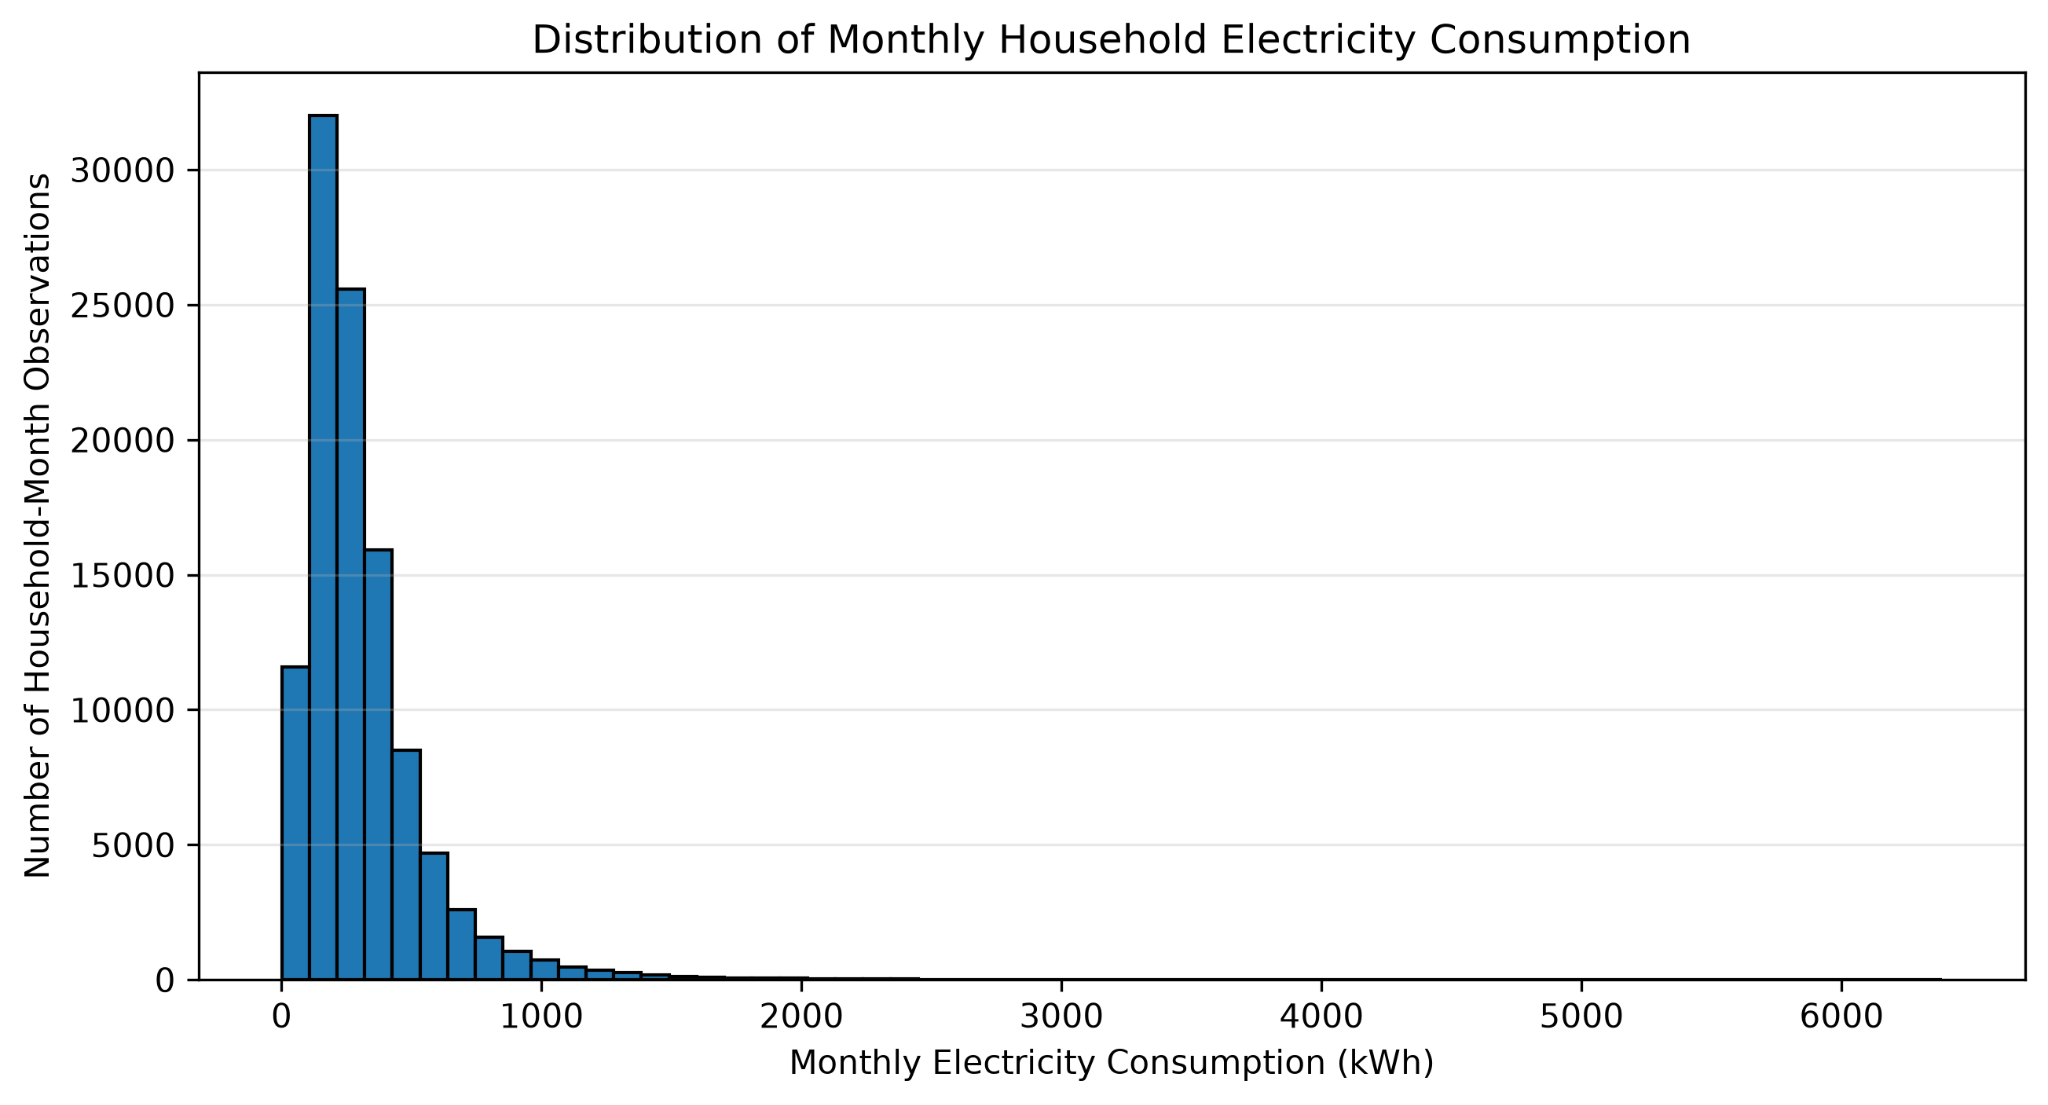
\includegraphics[width=.88\linewidth]{monthly_consumption_histogram.png}\caption{Distribution of monthly household electricity consumption.}\label{fig:hist}\end{figure}
\begin{figure}[H]\centering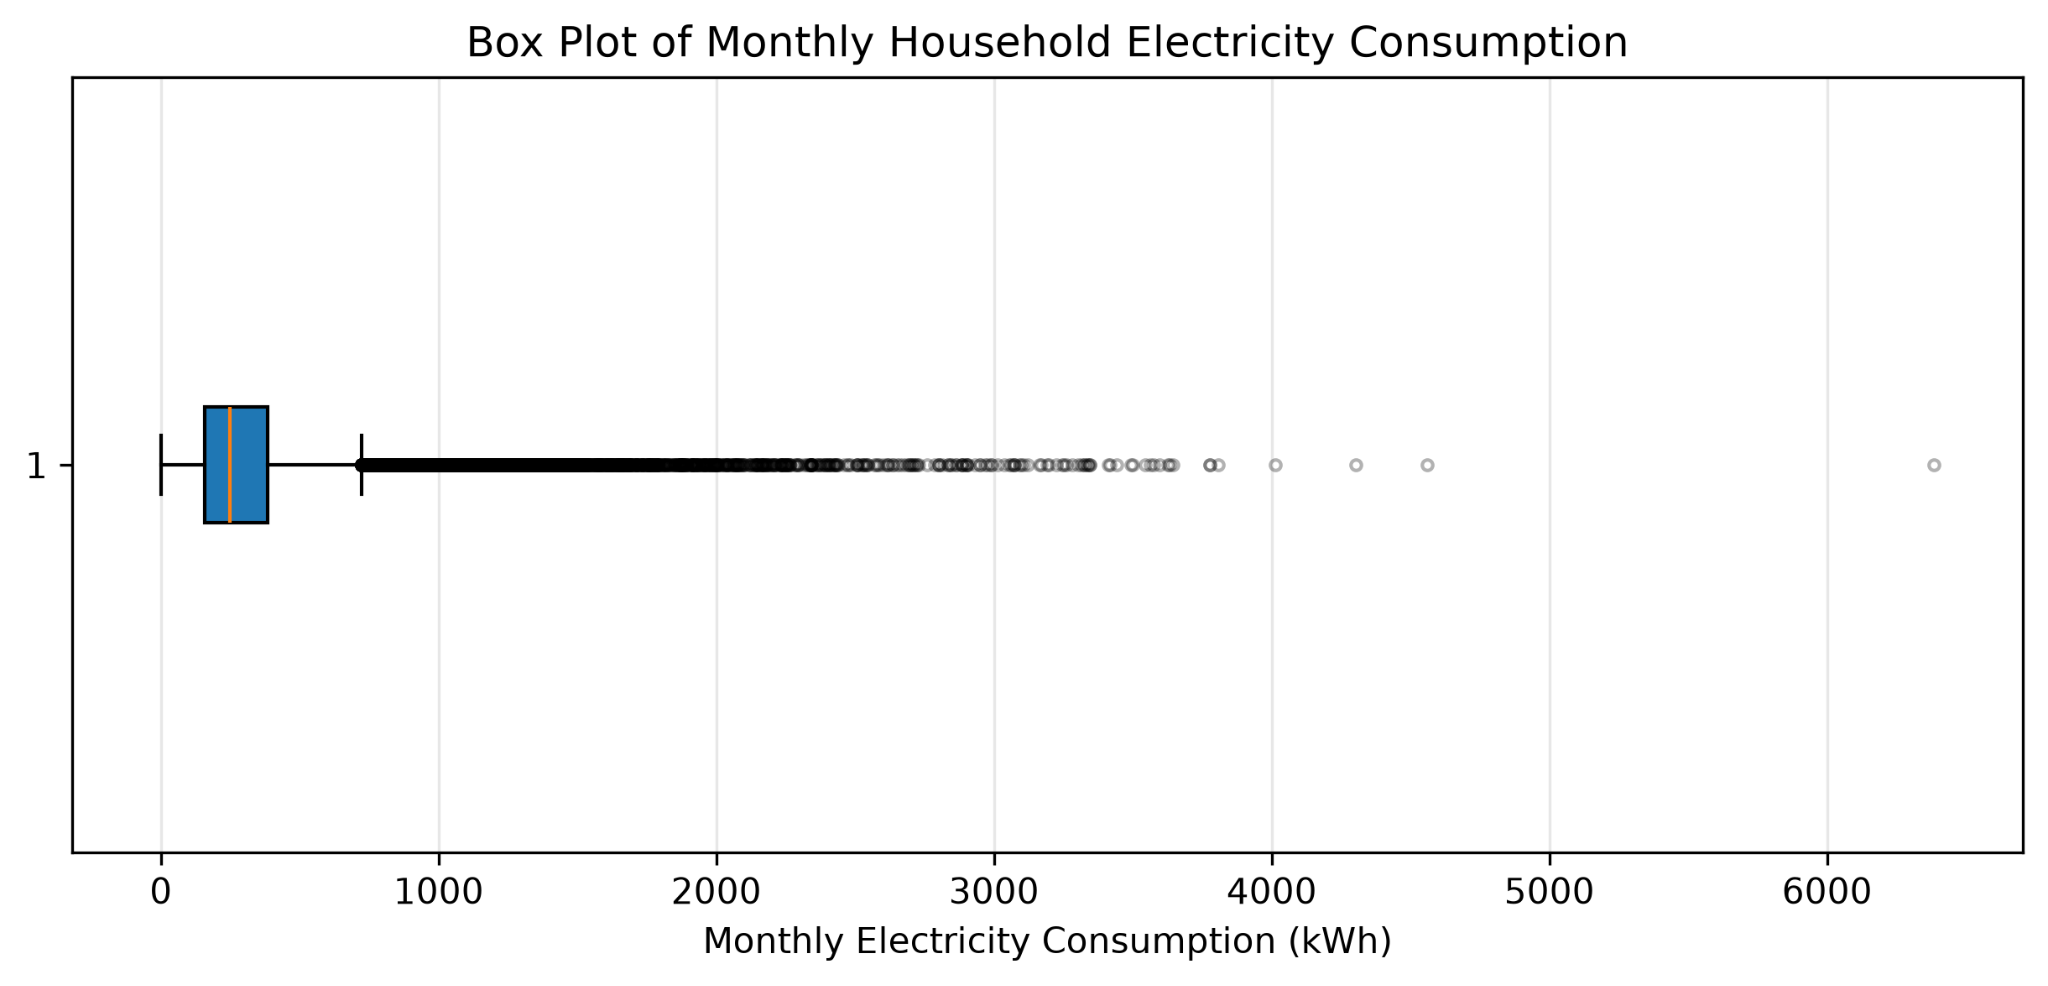
\includegraphics[width=.88\linewidth]{monthly_consumption_boxplot.png}\caption{Box plot of monthly household electricity consumption and potential high outliers.}\label{fig:box}\end{figure}
\subsection{Temporal and Seasonal Patterns}
Monthly consumption exhibited recurring seasonal variation, with higher electricity usage during colder months and lower usage during warmer months.

Average winter consumption was \textbf{373.13 kWh}, compared with \textbf{252.64 kWh} in summer, approximately 47.7\% higher. The correlation between monthly average temperature and aggregated average consumption was $-0.921$, indicating a strong negative relationship at the monthly aggregate level.
\begin{figure}[H]\centering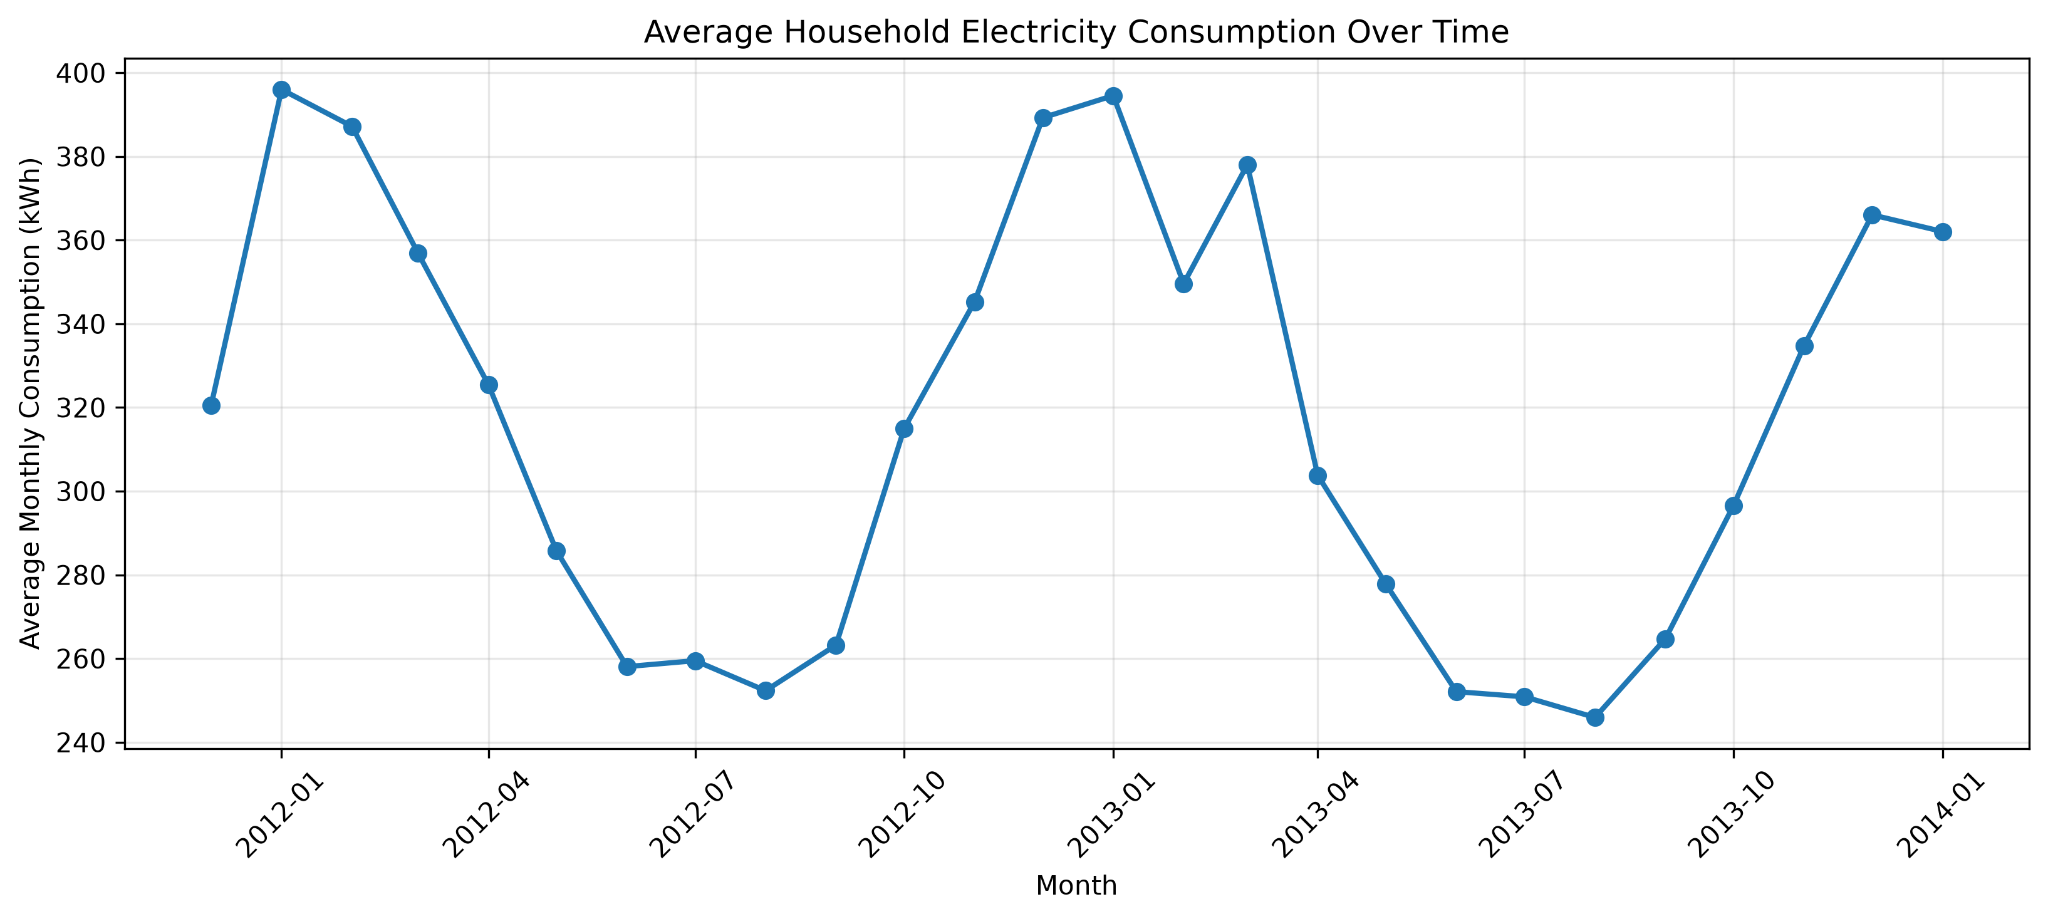
\includegraphics[width=.88\linewidth]{monthly_consumption_trend.png}\caption{Average household electricity consumption over time.}\label{fig:trend}\end{figure}
\begin{figure}[H]\centering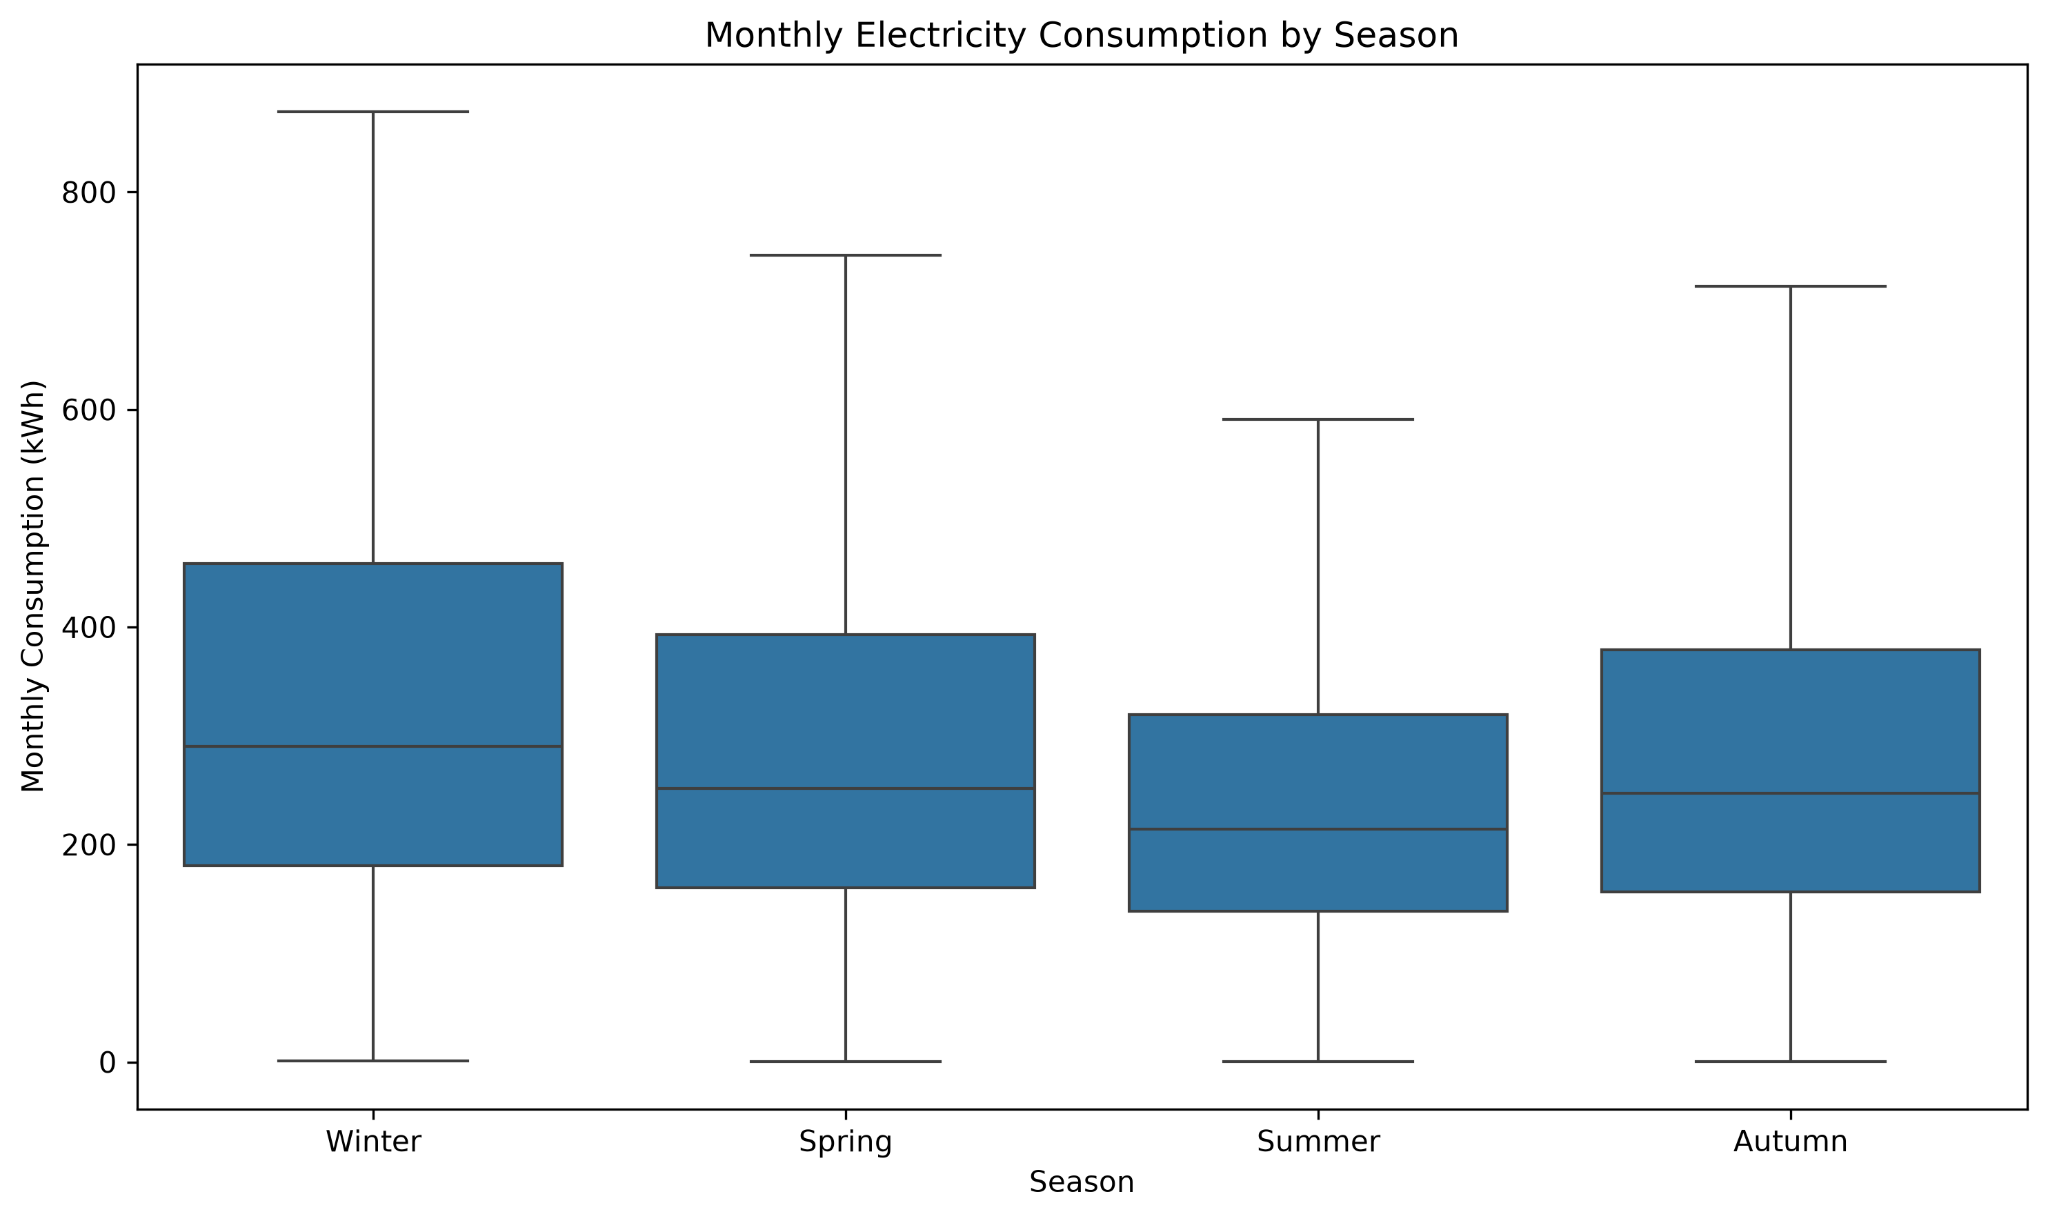
\includegraphics[width=.88\linewidth]{consumption_by_season.png}\caption{Distribution of monthly electricity consumption by season.}\label{fig:season}\end{figure}
\subsection{Relationships Among Variables}
Correlation analysis revealed a near-perfect positive relationship between monthly consumption and estimated bills, reflecting the bill calculation's dependence on electricity usage. At the household-month level, temperature showed a weaker negative correlation with consumption ($-0.187$).

Historical consumption features also demonstrated strong associations with estimated bills: previous-month consumption had a correlation of 0.928, while the three-month rolling average had a correlation of 0.878. However, these pooled relationships partly reflect differences between households.
\begin{figure}[H]\centering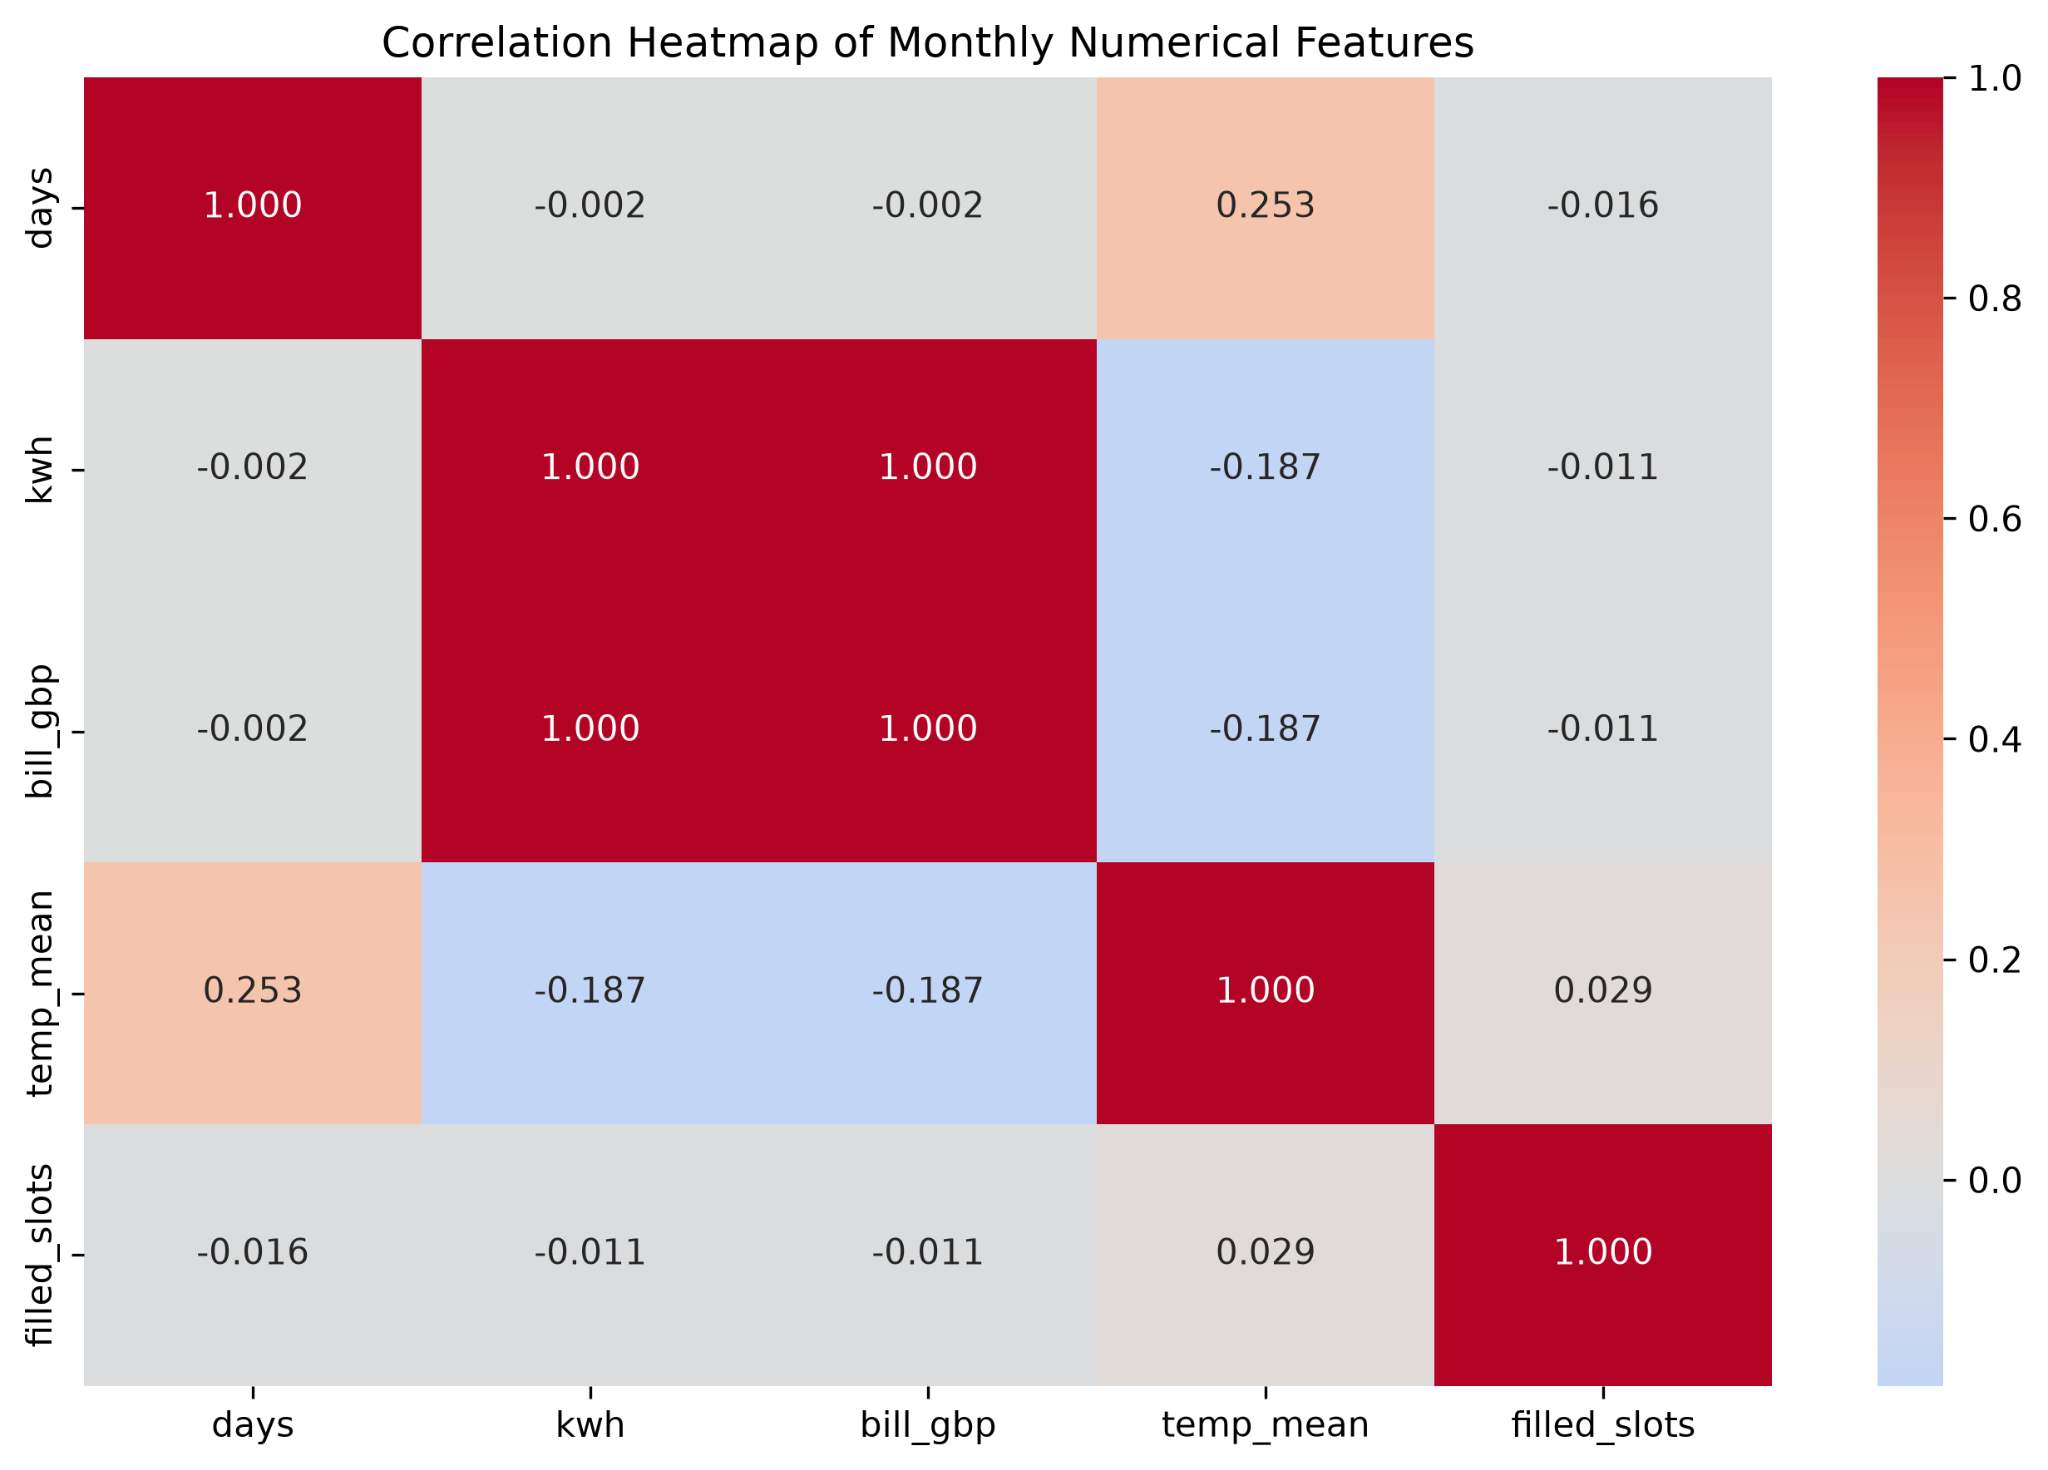
\includegraphics[width=.88\linewidth]{numerical_correlation_heatmap.png}\caption{Correlation heatmap of monthly numerical variables.}\label{fig:heat}\end{figure}
\subsection{Household and Tariff Differences}
Consumption varied across household classifications and tariff categories. Affluent ACORN households recorded the highest average consumption among the three principal ACORN groups (352.60 kWh), while Adversity households recorded the lowest (261.31 kWh).

Standard-tariff households averaged 315.96 kWh, compared with 291.16 kWh for Time-of-Use households. These differences are descriptive and do not establish causal relationships.
\subsection{Data Quality Considerations}
The analysis identified 292 gaps between consecutive household observations, affecting the availability of historical features. Duplicate checks confirmed that every household-month combination was unique. These findings informed the construction and validation of lagged and rolling consumption features.

\section{Key Insights and Modeling Implications}
The exploratory analysis revealed several patterns relevant to predicting household electricity bills. Table~\ref{tab:insights} summarizes the principal findings and their implications for model development.
\begin{table}[H]\centering\caption{Key insights and modeling implications}\label{tab:insights}\footnotesize
\begin{tabular}{@{}p{.44\linewidth}p{.48\linewidth}@{}}\toprule
Key insight & Modeling implication\\\midrule
Seasonal variation: winter consumption was approximately 47.7\% higher than summer consumption. & Include calendar and seasonal features to capture recurring consumption patterns.\\
Historical consumption: previous-month and three-month rolling consumption correlated with bills (0.928 and 0.878). & Use historical consumption features as potential predictors.\\
Household differences: ACORN consumption varied; within-household correlations were weaker than pooled correlations. & Retain household classification features and evaluate performance across households.\\
Skewness and outliers: 5.46\% exceeded the IQR upper boundary. & Consider robust preprocessing and models capable of handling extreme values.\\
Temperature: monthly aggregate correlation with consumption was $-0.921$. & Consider weather information available at prediction time.\\
Historical data gaps reduced lag and rolling feature availability. & Account for missing historical features during model development.\\
Historical features were highly correlated (0.957). & Examine redundancy and compare contributions during evaluation.\\\bottomrule
\end{tabular}\end{table}
\subsection{Implications for Forecasting}
These findings suggest that historical electricity consumption, seasonal patterns, and household characteristics are promising inputs for monthly bill prediction. However, strong pooled correlations do not guarantee equally strong predictive performance for individual households.

Furthermore, the near-perfect relationship between current-month consumption and estimated bills highlights the importance of preventing target leakage. Features that become available only after the prediction period must not be used to forecast that period's bill.

Consequently, subsequent modeling will focus on information available before the target billing period, with appropriate treatment of missing historical values and feature scaling where required.

\section{Feature Engineering}
Feature engineering introduced attributes that capture historical electricity consumption and seasonal patterns. The process extended the previously encoded dataset from 15 to 23 columns while preserving all 106,225 observations.
\subsection{Newly Engineered Features}
Eight features were created during Phase 3, as summarized in Table~\ref{tab:features}.
\begin{table}[H]\centering\caption{Engineered features, descriptions, and justifications}\label{tab:features}\footnotesize
\begin{tabular}{@{}p{.28\linewidth}p{.31\linewidth}p{.33\linewidth}@{}}\toprule
Feature & Description & Justification\\\midrule
\texttt{previous\_month\_kwh} & Consumption in the preceding calendar month & Captures recent household behavior.\\
\texttt{rolling\_3month\_kwh} & Mean of preceding three consecutive calendar months & Captures trends and smooths short-term fluctuations.\\
\texttt{month\_number} & Calendar month (1--12) & Represents recurring monthly patterns.\\
\texttt{quarter} & Calendar quarter (1--4) & Captures broader seasonal periods.\\
\texttt{season\_winter} & Indicator for December--February & Identifies winter patterns.\\
\texttt{season\_spring} & Indicator for March--May & Identifies spring patterns.\\
\texttt{season\_summer} & Indicator for June--August & Identifies summer patterns.\\
\texttt{season\_autumn} & Indicator for September--November & Identifies autumn patterns.\\\bottomrule
\end{tabular}\end{table}
Historical features were calculated using preceding calendar months only, preventing current-month consumption from entering their calculations.
\subsection{Previously Encoded Categorical Features}
Five categorical indicators created during Phase 2 were retained: \texttt{tariff\_tou}, \texttt{acorn\_affluent}, \texttt{acorn\_comfortable}, \texttt{acorn\_adversity}, and \texttt{acorn\_unknown}.

These represent electricity tariff categories and household socioeconomic classifications. They were not regenerated during Phase 3 but remain potential predictors because tariff information affects billing calculations and household characteristics may help explain consumption differences.
\subsection{Feature Availability and Validation}
Historical feature availability was assessed to identify limitations caused by incomplete household consumption histories.
\begin{table}[H]\centering\caption{Historical feature availability}\small
\begin{tabular}{@{}lrrr@{}}\toprule
Feature & Available & Missing & Availability\\\midrule
\texttt{previous\_month\_kwh} & 100,385 & 5,840 & 94.50\%\\
\texttt{rolling\_3month\_kwh} & 88,947 & 17,278 & 83.73\%\\\bottomrule
\end{tabular}\end{table}
Missing values arise primarily from initial household observations and gaps in consecutive monthly records. These values were retained rather than imputed during this phase.

Validation confirmed that the engineered dataset contained no duplicate household-month records and that each observation belonged to exactly one season.
\subsection{Feature Selection and Scaling}
The engineered historical and calendar features, together with previously encoded tariff and ACORN indicators, were retained as candidate predictors.

Current-month total consumption (\texttt{kwh}) and actual current-month temperature were excluded from the advance forecasting feature set because their complete values would not be available at prediction time. Household identifiers and other administrative fields were also not treated as direct numerical predictors.

Given the skewed consumption distributions and extreme values observed during EDA, robust scaling may be appropriate for models sensitive to feature magnitude. However, scaling was deferred until model development, when parameters can be estimated using training data only to prevent information leakage.

The resulting dataset was saved as \texttt{data/processed/monthly\_features.parquet}, containing 23 columns and 106,225 household-month observations.
\section{Conclusion}
This phase examined monthly household electricity consumption through exploratory data analysis and feature engineering. The findings revealed seasonal consumption patterns, substantial differences across households, strong relationships between historical consumption and estimated bills, and positively skewed distributions with potential outliers.

Eight additional features were engineered to capture historical consumption and calendar-based patterns, while previously encoded tariff and household classification features were retained. The resulting dataset contains \textbf{106,225 household-month observations and 23 columns}, with validation confirming the uniqueness of household-month records.

These findings provide a foundation for the next phase of the project, which will focus on developing and evaluating models for predicting household electricity bills using information available before the target billing period.
\end{document}
